\def\UseMinted{}
\documentclass[../main.tex]{subfiles}
\begin{document}
	
	
\section{Rozwiązanie}
Nasze rozwiązanie obejmuje platformę symulacyjną Risc-v-simple w SIMICS z systemem linux oraz programem skompilowanym z sanitizerem. Do programu celowo wprowadziliśmy błędny dostęp do pamięci.

\subsection{Linux}

\subsubsection{Sterownik}
Napisaliśmy prosty sterownik (moduł jądra Linux) do obsługi bufora na wyjście sanitizera. Moduł ten pozwala nam na wpisywanie ciągów znaków do zdefiniowanego przez nas obszaru pamięci w celu ich późniejszego odczytania przez emulator SIMICS.


\subsubsection{External-buildroot}
Stworzyliśmy external-repository w buildroot w celu budowania naszego modułu dla jądra linuxa.

\subsubsection{Modyfikacja Device-Tree}
	Do drzewa urządzeń dodaliśmy własne urządzenie (simics_shm), które jest buforem pamięci.
	\begin{listing}
		\begin{minted}[highlightlines={}]{sh}
simics_shm: simics_shm@20000000 {
	compatible = "simics_shm";
	device_type = "memory";
	reg = <0x00 0x20000000 0x00 0x4000>;
	status = "open";
};
		\end{minted}
	\end{listing}
	Następnie zmodyfikowane drzewo urządzeń budujemy do postaci binarnej, poleceniem 
	
	\begin{listing}
		\begin{minted}[highlightlines={}]{sh}
dtc -O dtb -o risc-v-simple.dtb risc-v-simple.dts
		\end{minted}
	\end{listing}


\subsubsection{Overlay dla buildroot}
Overlay w buildroot do dołączania programów lub plików do platformy docelowej do systemu plików. Wydał nam się najszybszym sposobem na statyczne osadzenie naszego programu w systemie. Głównie dlatego, że go już znaliśmy.

\subsubsection{Budowanie systemu}
Budowaliśmy system Linux, jak już wcześniej wspomniano korzystając z Buildroota i dodając mu odpowiednie flagi służące do obsługi externala oraz overleya.

\subsubsection{Dodawanie systemu do SIMICS}
Wgranie zbudowanego systemu do platformy emulowanej można wykonać poprzez (i tak to zrobiliśmy), np. poprzez linkowanie plików wynikowych z budowania systemów w buildroot do folderu targets w platformie risc-v-simple w SIMICS, wykonaliśmy to poleceniem:
	\begin{listing}
		\begin{minted}[highlightlines={}]{sh}
ln -r -s ~/buildroot/output/images/* \
~/simics/simics-risc-v-simple-7.x.x/...
...targets/risc-v-simple/images/linux/
		\end{minted}
	\end{listing}
Dzięki temu nasza platforma po przebudowaniu będzie widoczna w aktualnej wersji z poziomu SIMICS, bez potrzeby ponownego kopiowania plików.



\subsection{SIMICS (i jego konfiguracja)}
\subsubsection{Dodawanie urządzenia}
Aby dodać urządzenie w emulatorze, aby adresy pamięci podane w naszym sterowniku były poprawnie intepretowane przez SIMICS i jądro linuxa, stworzylismy każdorazowo obiekt:
	\begin{listing}
		\begin{minted}[highlightlines={}]{simics}
fb_img = simics.SIM_create_object(
	"ram", f"{fb_ns}.buffer", image=None,
	self_allocated_image_size=size_bytes)
		\end{minted}
	\end{listing}
\subsubsection{Skrypt inicjujący platformę}
Aby nie podawać za każdym razem kilku komend związanych z utworzeniem obiektu naszej pamięci oraz ładowania platformy, napisaliśmy skrypt:
	\begin{listing}
	\begin{minted}[highlightlines={}]{sh}
load-target "risc-v-simple/linux"
@SIM_create_object("ram","board.sanitizer_shm", image=None, self_allocated_image_size=0x1000)
board.phys_mem.add-map board.sanitizer_shm 0x20000000 0x1000
	\end{minted}
\end{listing}

\subsubsection{Python MAGIC -- hook}
Napisaliśmy też skrypt w języku python do uruchamiania w SIMICS, aby przechwtywać MAGIC instructions.
	\begin{listing}
	\begin{minted}[highlightlines={}]{sh}
def branch():
	while True:
		conf.bp.magic.cli_cmds.wait_for(number=MAGIC_NUMBER)
		print("asan: ", end="")
		addr = SANITIZER_SHM_ADDR
		while True:
			byte = conf.board.phys_mem.memory[addr]
			if byte == 0:
				break
			print(chr(byte), end="")
			if byte == 10:
				print("asan: ", end="")
			addr += 1
		print()
	\end{minted}
\end{listing}

\subsection{Kompilacja programu}



\subsubsection{Program bad.c}
IG WYMAGA KOMENTARZA
\begin{listing}
	\begin{minted}[highlightlines={}]{c}
	int main(int argc, char **argv)
	{
		volatile int a[5] = {0};
		a[6] = argc;
		return 0;
	}
	
	\end{minted}
\end{listing}


\subsubsection{Nakładka na libsan}
IG WYMAGA KOMENTARZA
	\begin{listing}
	\begin{minted}[highlightlines={}]{c}
#define MAGIC_NUMBER 28
void __sanitizer_on_print(const char *str){...}
MAGIC(MAGIC_NUMBER);		
	\end{minted}
\end{listing}


\subsubsection{Stworzenie wynikowego pliku bad.elf}
KOMENTARZ
	\begin{listing}
	\begin{minted}[highlightlines={}]{sh}
$(MAKE) -C libsan-overlay
$(MAKE) -C bad-program
$(LD) -o $(BAD_PATCHED_O) -r bad-program/bad.o libsan-overlay/libsan-overlay.o
$(CC) -o $(TARGET) $(BAD_PATCHED_O) -static-libasan -fsanitize=address
	\end{minted}
\end{listing}


\subsection{Uruchomienie platformy (demonstracja działania)}

\begin{enumerate}
	\item Budowanie systemu
	\item Budowanie aplikacji z sanitizerem (i błędem)
	
	\item Uruchomienie SIMICS, a w emulatorze:
	\begin{enumerate}
		\item uruchamiamy skrypt Python (magic-hook.py)
		
		\item ładujemy platformę (skrypt map\_memory.simics)
		\item uruchamiamyy system (polecenie: run)
		
		\item Uruchomienie programu: ./bad
		
		\item Obserwacja wyników:
		
	\end{enumerate}
\end{enumerate}

\begin{figure}
	\centering
	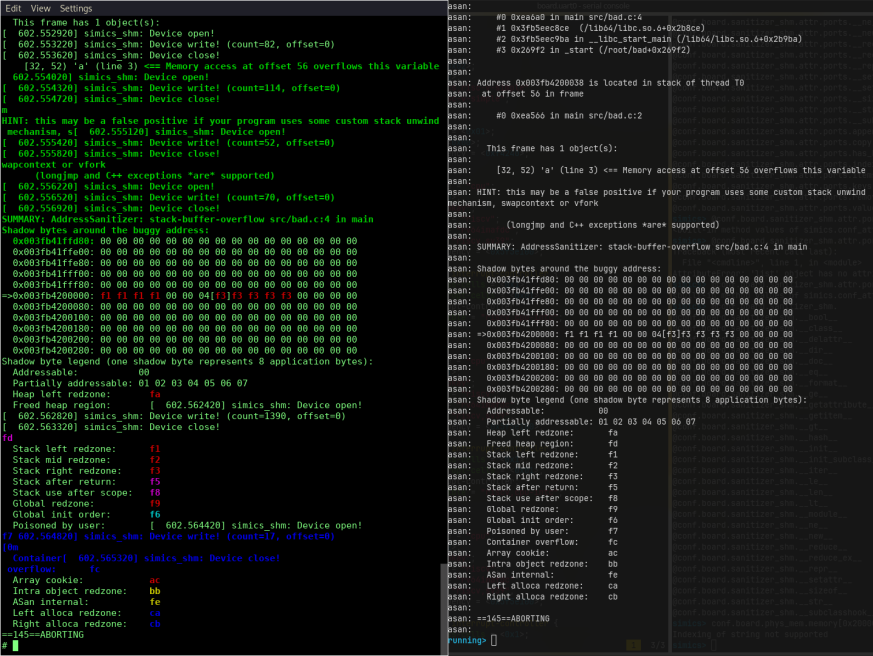
\includegraphics[width=0.7\linewidth]{images/end}
	\caption{Końcowy rezultat projektu - uruchomiony SIMICS, w nim Linux i nasz program z sanitizerem. Widać, że print sanitizera udało się przenieść do terminala z emulatorem}
	\label{fig:end}
\end{figure}

\end{document}